\documentclass[a4paper]{article}

\usepackage{amsmath}
\usepackage{amssymb}
\usepackage{parskip}
\usepackage{fullpage}
\usepackage{hyperref}
\usepackage{tikz}
\usepackage{fancybox}
\usepackage{makecell}

\hypersetup{
    colorlinks=true,
    linkcolor=black,
    urlcolor=blue,
    pdftitle={Merkle Tree},
    pdfpagemode=FullScreen,
}

\title{Merkle Tree}
\author{Paolo Bettelini}
\date{}

\begin{document}

\maketitle
\tableofcontents
\pagebreak

\section{Definition}

\begin{center}
    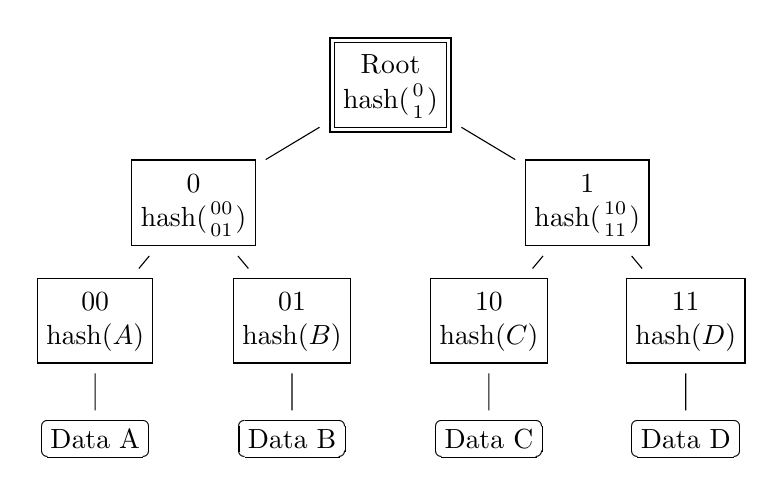
\begin{tikzpicture}[
        level 1/.style = {sibling distance = 5cm},
        level 2/.style = {sibling distance = 2.5cm}
    ]
    \node {\doublebox{\makecell{Root \\ \(\text{hash}({0\atop 1})\) }}}
        child {
            node {\fbox{\makecell{0 \\ \(\text{hash}({00\atop 01})\) }}}
            child {
                node {\fbox{\makecell{00 \\ \(\text{hash}(A)\) }}}
                child {
                    node {\ovalbox{Data A}}
                }
            }
            child {
                node {\fbox{\makecell{01 \\ \(\text{hash}(B)\) }}}
                child {
                    node {\ovalbox{Data B}}
                }
            }
        }
        child {
            node {\fbox{\makecell{1 \\ \(\text{hash}({10\atop 11})\) }}}
            child {
                node {\fbox{\makecell{10 \\ \(\text{hash}(C)\) }}}
                child {
                    node {\ovalbox{Data C}}
                }
            }
            child {
                node {\fbox{\makecell{11 \\ \(\text{hash}(D)\) }}}
                child {
                    node {\ovalbox{Data D}}
                }
            }
        };
    \end{tikzpicture}
\end{center}

A Markle tree or hash tree is a tree where each node contains the hash
of its children, and every leaf contains the hash of a data block.


\pagebreak

\end{document}
